\documentclass{article}

% Language setting
% Replace `english' with e.g. `spanish' to change the document language
\usepackage[english]{babel}

% Set page size and margins
% Replace `letterpaper' with `a4paper' for UK/EU standard size
\usepackage[letterpaper,top=2cm,bottom=2cm,left=3cm,right=3cm,marginparwidth=1.75cm]{geometry}

% Useful packages
\usepackage{amsmath}
\usepackage{graphicx}
\usepackage[colorlinks=true, allcolors=blue]{hyperref}
\usepackage{textgreek}
\usepackage{verbatim}
\usepackage{caption}
\usepackage{subcaption}
\usepackage{float}
\usepackage{array}
\usepackage{listings}
\usepackage{xcolor}
\usepackage{natbib}
\usepackage{hyperref}

\pdfinfo{
  /Title (RFID-RC522 Key Reading)
  /Author (Abel Haro Armero)
  /Subject (Internet of Things)
}


\begin{document}

\definecolor{background}{rgb}{0.95,0.95,0.92}  % Light gray background color

\lstset{ 
  language=Python,                % the language of the code
  basicstyle=\ttfamily\small,     % the size of the fonts that are used for the code
  numbers=left,                   % where to put the line-numbers
  numberstyle=\tiny\color{gray},  % the style that is used for the line-numbers
  stepnumber=1,                   % the step between two line-numbers. If it's 1, each line will be numbered
  numbersep=5pt,                  % how far the line-numbers are from the code
  backgroundcolor=\color{white},  % choose the background color. You must add \usepackage{color}
  showspaces=false,               % show spaces adding particular underscores
  showstringspaces=false,         % underline spaces within strings
  showtabs=false,                 % show tabs within strings adding particular underscores
  frame=single,                   % adds a frame around the code
  rulecolor=\color{black},        % if not set, the frame-color may be changed on line-breaks within not black text (e.g. comments (green here))
  tabsize=2,                      % sets default tabsize to 2 spaces
  captionpos=b,                   % sets the caption-position to bottom
  breaklines=true,                % sets automatic line breaking
  breakatwhitespace=false,        % sets if automatic breaks should only happen at whitespace
  title=\lstname,                 % show the filename of files included with \lstinputlisting; also try caption instead of title
  keywordstyle=\color{blue},      % keyword style
  commentstyle=\color{gray},      % comment style, changed to magenta for better readability
  stringstyle=\color{red},        % string literal style
  escapeinside={\%*}{*)},         % if you want to add LaTeX within your code
  morekeywords={*,...}            % if you want to add more keywords to the set
}


\begin{titlepage}
\centering
{\bfseries\LARGE Universidad Politécnica de Valencia\par}
\vspace{1cm}
{\scshape\Large Escuela Técnica Superior de Ingeniería Informática\par}
\vspace{3cm}
{\scshape\Huge RFID-RC522 Key Reading\par}
\vspace{3cm}
{\itshape\Large Internet of Things\par}
\vfill
{\Large Abel Haro Armero\par}
\vfill
{\Large June 2024\par}
\date{}
\end{titlepage}

\tableofcontents

\newpage


\section{Introduction}

This project involves developing an access control system using RFID technology (RFID-RC522 reader).
The system will allow user registration and access control using RFID keys and cards. 
To switch the reader mode between registration and access, Bluetooth communication will be used. 
Registered users and accesses will be stored in a database accessible via a REST API within a container. 
For visualization, Ubidots will be used.
The entire project is available in a GitHub repository \href{https://github.com/AbelHaro/RFID-RC522-Key-Reading}{RFID-RC522 Key Reading} \cite{abelharo2024lectura}.

\begin{figure}[H]
\centering
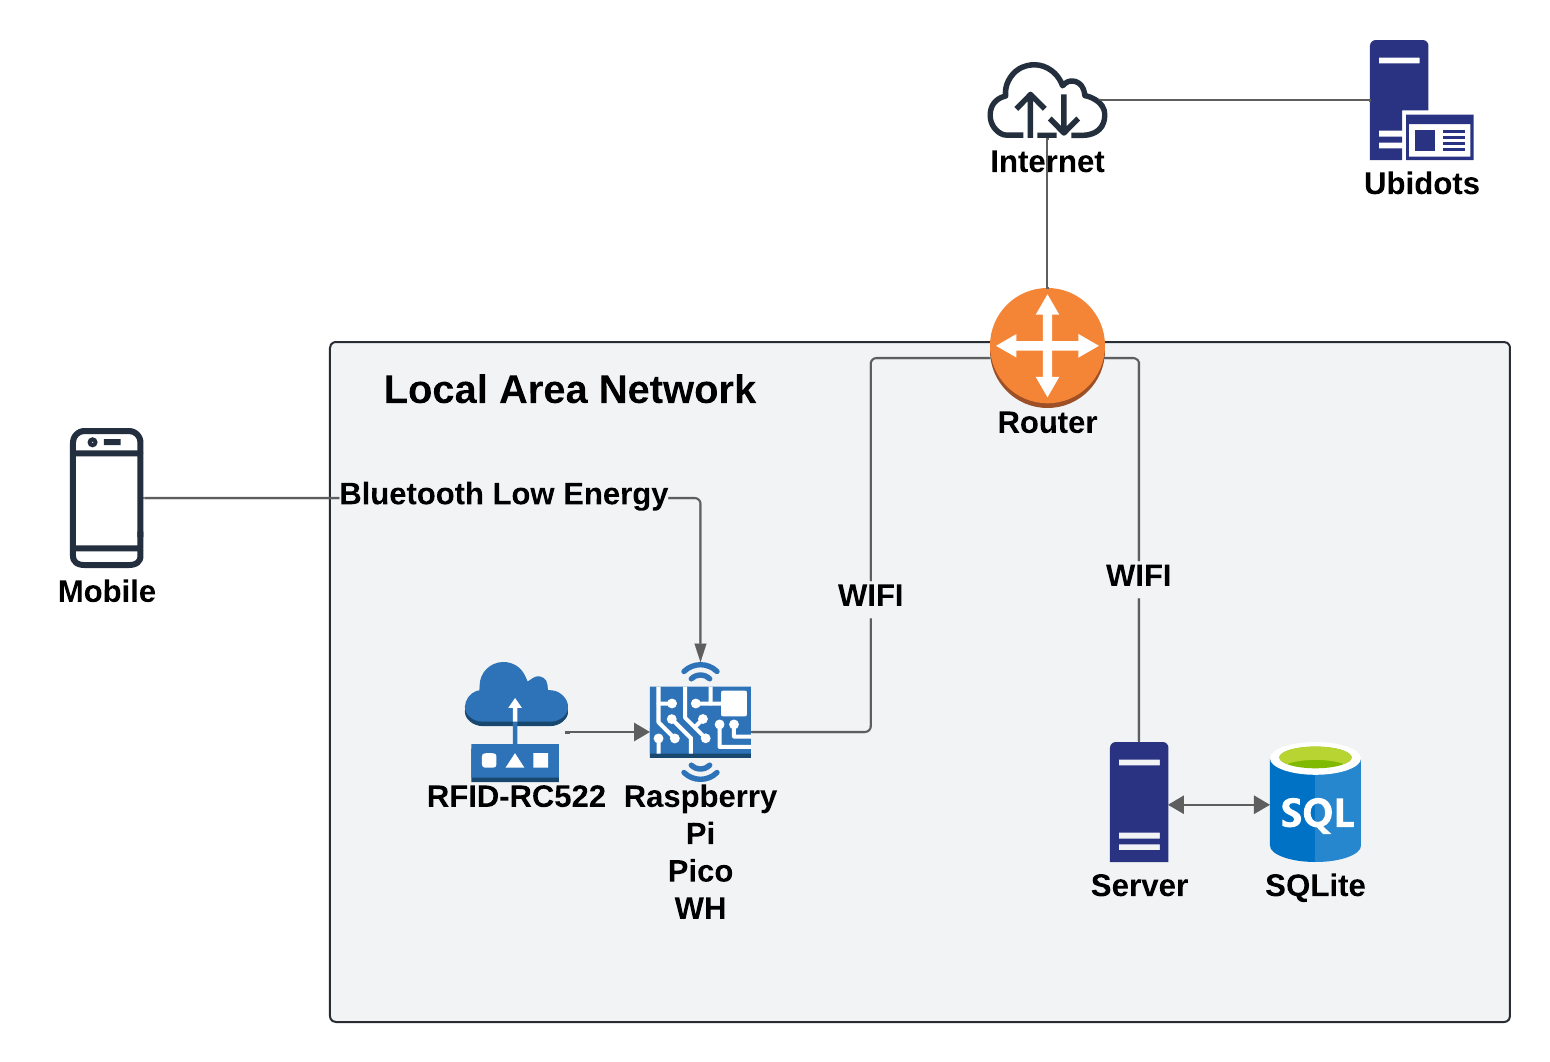
\includegraphics[width=0.9\linewidth]{../images/esquema_proyecto.png}
\caption{\label{fig:esquema red}Project diagram.}
\end{figure}

\section{Hardware Used}
The following hardware was used for the project:

\begin{figure}[H]
	\centering
	\begin{subfigure}[b]{0.45\textwidth}
		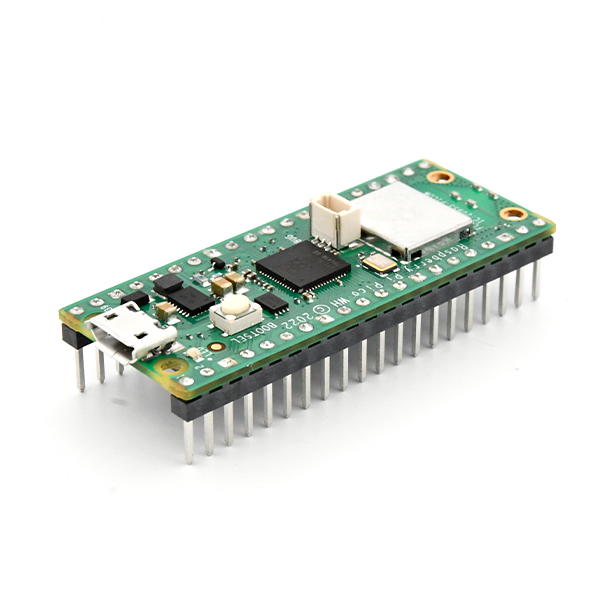
\includegraphics[width=\textwidth]{../images/picowh.png}
		\caption*{\href{https://www.raspberrypi.com/products/raspberry-pi-pico/}{Raspberry Pi Pico WH Microcontroller}}
		\label{fig:picowh}
	\end{subfigure}
	\hfill
	\begin{subfigure}[b]{0.45\textwidth}
		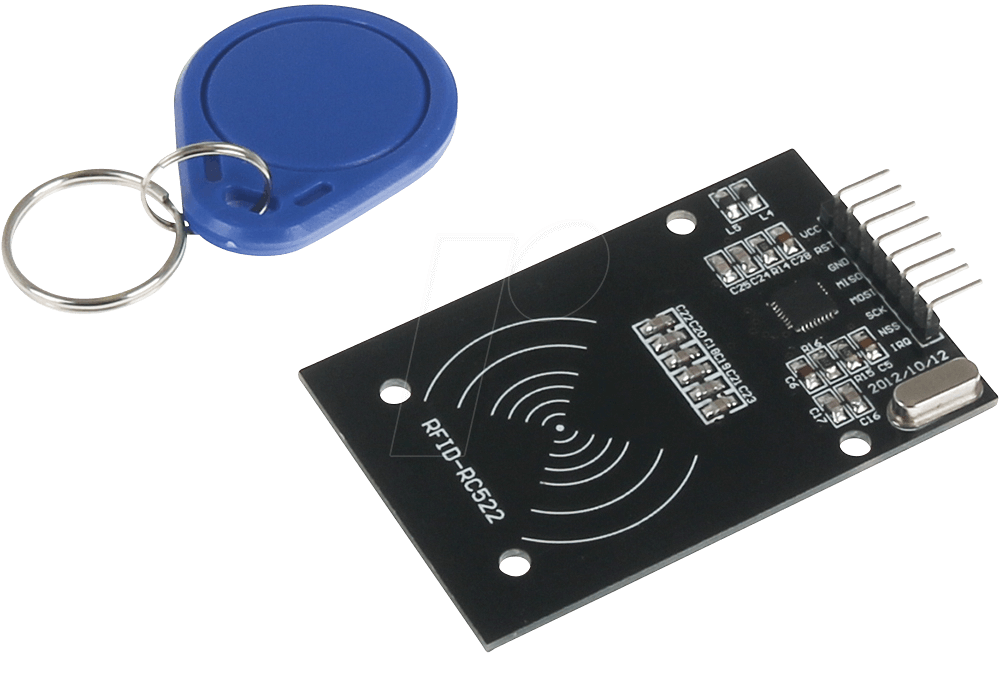
\includegraphics[width=\textwidth]{../images/mfrc522.png}
		\caption*{\href{https://www.keyestudio.com/products/keyestudio-mfrc522-rfid-s50-fudan-card-ic-card-module-with-spi-port-for-arduino-uno-r3-mega-2560-r3}{RFID-RC522 Radio Frequency Reader}}
		\label{fig:MFRC522}
	\end{subfigure}
\end{figure}

\begin{figure}[H]
	\centering
	\begin{subfigure}[b]{0.45\textwidth}
		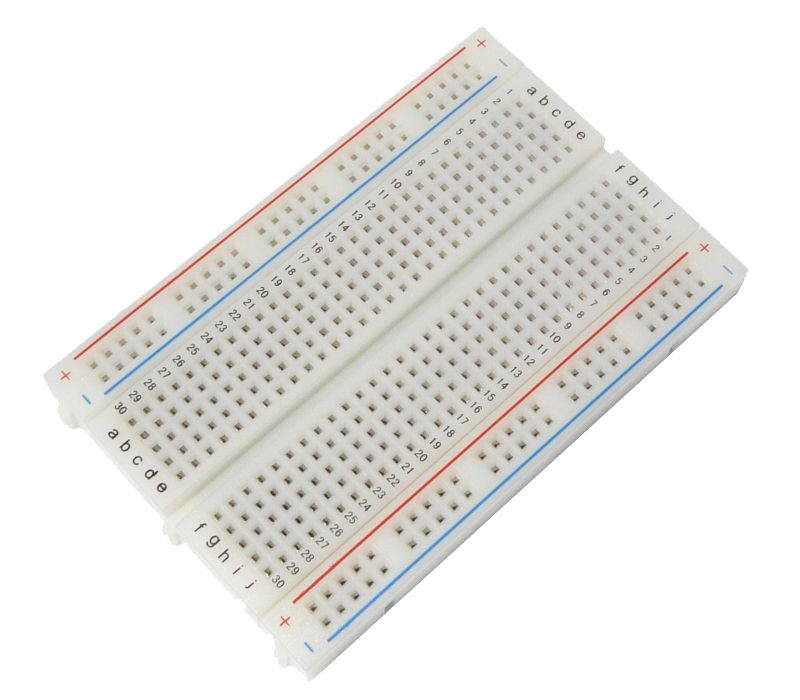
\includegraphics[width=\textwidth]{../images/protoboard.png}
		\caption*{Protoboard}
		\label{fig:protoboard}
	\end{subfigure}
	\hfill
	\begin{subfigure}[b]{0.45\textwidth}
		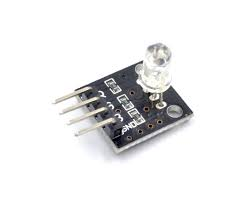
\includegraphics[width=\textwidth]{../images/led_tricolor.jpg}
		\caption*{Tri-color LED KY-016 SP00}
		\label{fig:led tricolor}
	\end{subfigure}
\end{figure}

\begin{figure}[H]
	\centering
	\begin{subfigure}[b]{0.3\textwidth}
		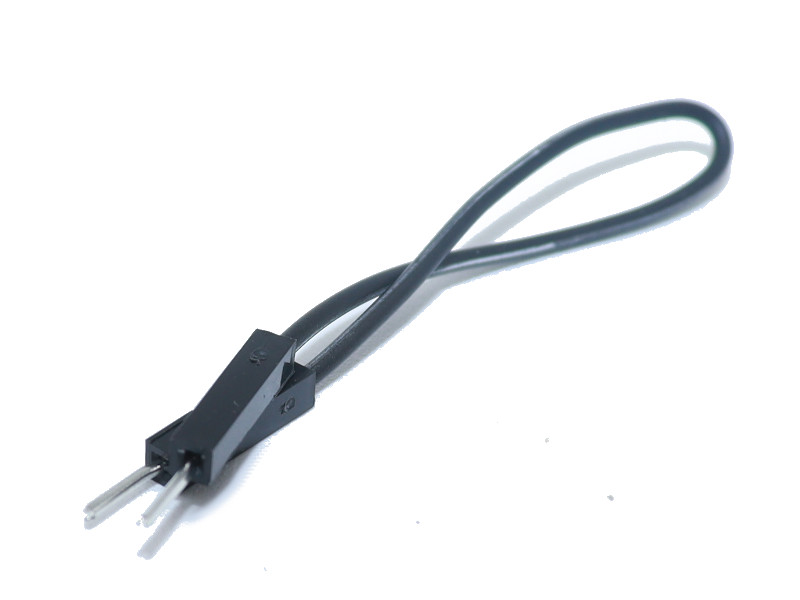
\includegraphics[width=\textwidth]{../images/cable_mm.jpg}
		\caption*{Dupont Male-Male Cable x3}
		\label{fig:cable mm}
	\end{subfigure}
	\hfill
	\begin{subfigure}[b]{0.3\textwidth}
		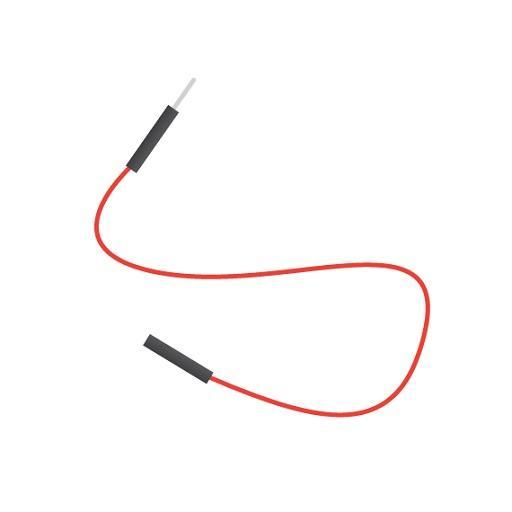
\includegraphics[width=\textwidth]{../images/cable_mh.jpg}
		\caption*{Dupont Female-Male Cable x5}
		\label{fig:cable mh}
	\end{subfigure}
	\hfill
	\begin{subfigure}[b]{0.3\textwidth}
		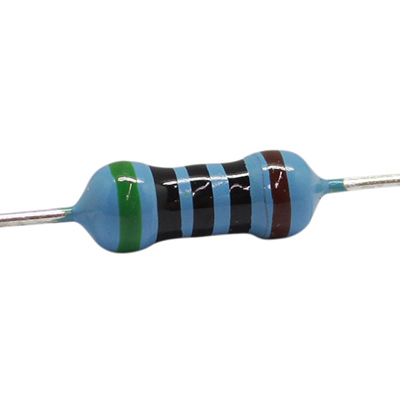
\includegraphics[width=\textwidth]{../images/resistencia.jpg}
		\caption*{500\textOmega\ Resistor x2}
		\label{fig:resistencia}
	\end{subfigure}
\end{figure}


\section{Software Used}
The following software was used for the project.
\subsection{Microcontroller}
MicroPython was used as the programming language for the Raspberry Pi Pico WH microcontroller.
To establish and manage Bluetooth communication on the microcontroller, the \href{https://github.com/micropython/micropython/tree/master/examples/bluetooth}{BLE (Bluetooth Low Energy) libraries} \cite{micropythonBluetoothExamples} were utilized.
For the mobile device, the \href{https://play.google.com/store/apps/details?id=de.kai_morich.serial_usb_terminal&pcampaignid=web_share}{Serial Bluetooth Terminal} app \cite{sam2023ble} available on Play Store was used. For reading RFID keys and cards, the \href{https://github.com/danjperron/micropython-mfrc522/blob/master/mfrc522.py}{MFRC522 library} \cite{danjperron2022mfrc522} was employed.
In communication with the server, a REST API was implemented to enable structured data exchange. Finally, the standard machine library was used to turn LEDs on and off.

\subsection{Server}
For the server implementation, a Docker container with the base image of Ubuntu was used. 
Python was installed on the image along with the Flask package to manage server logic through HTTP requests. 
For data persistence, a Docker volume was used along with an SQLite database.
For server development, the code from the \href{https://pmanzoni.notion.site/LAB-6-REST-d487dab1b7e24d56b31d8e552a480888}{Lab 6 - REST} \cite{manzoni2024lab6} was modified.

\subsection{Ubidots}
The \href{https://stem.ubidots.com/}{Ubidots} platform was used for visualization through a STEM account. Ubidots allows real-time data visualization with a request rate of 1 req/s.

\section{Steps to Complete the Project}
The following steps should be followed to complete the project.
\subsection{Step 1: Pre-installation of Necessary Software}
\textbf{Server Application Installations:}
\begin{enumerate}
    \item Install \href{https://thonny.org/}{Thonny}.
    \item Install \href{https://code.visualstudio.com/download}{Visual Studio Code}.
    \item Install \href{https://docs.docker.com/get-docker/}{Docker}.
    \item Install \href{https://kinsta.com/es/base-de-conocimiento/instalar-python/}{Python interpreter}.
\end{enumerate}


\textbf{File Installation on Raspberry Pi Pico WH:}
\begin{enumerate}
	\item Install MicroPython firmware:
		\begin{enumerate}
			\item Insert the USB into the computer while pressing the BOOTSEL button.
			\item Open Thonny and follow these steps:
			\begin{figure}[H]
			\centering
			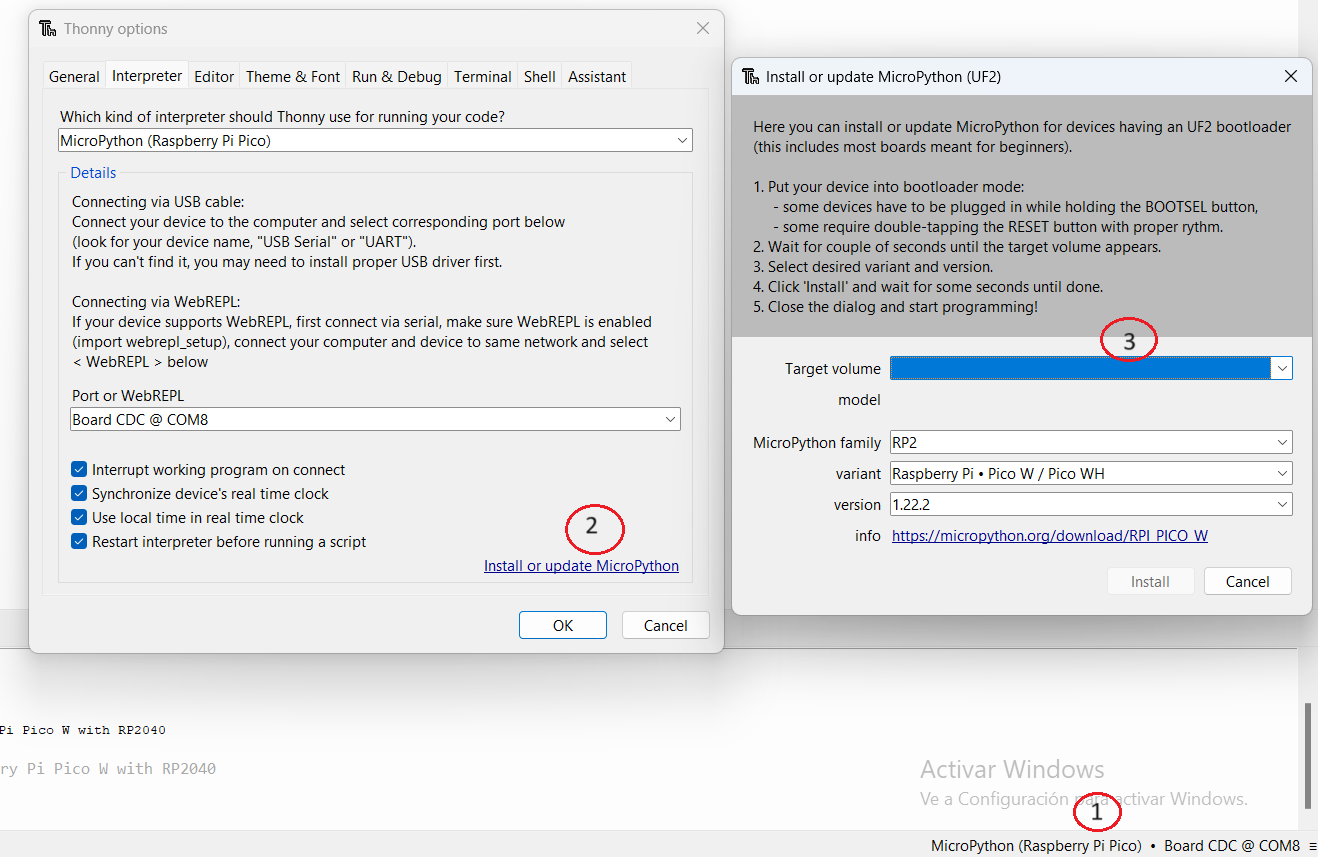
\includegraphics[width=0.8\linewidth]{../images/instalacion_firmware.png}
			\caption{\label{fig:instalación firmware}Steps to install the firmware.}
			\end{figure}
		\end{enumerate}
			\item Copy the contents of the \texttt{``microcontroller''} folder from the project to the Raspberry Pi Pico WH.
			\item Configure the \texttt{``ssid''} and \texttt{``password''} variables inside the \texttt{``microcontroller/wifi\_connect.py''} file with your network's \texttt{ssid} and \texttt{password}.
\end{enumerate}

\textbf{Ubidots Registration and Configuration:}
\begin{enumerate}
	\item Create an account on \href{https://stem.ubidots.com/}{Ubidots Stem}.
	\item Create a new device.
	\begin{figure}[H]
		\centering
		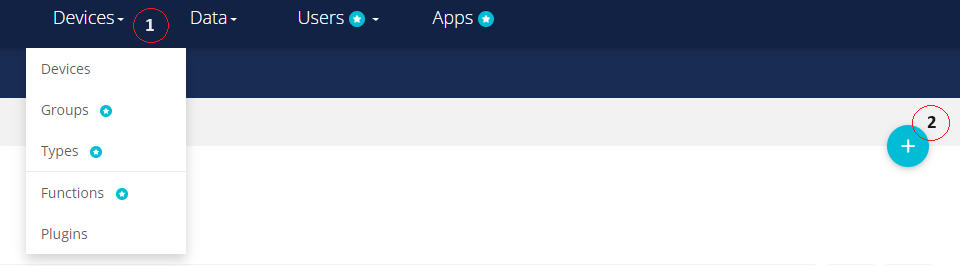
\includegraphics[width=0.7\linewidth]{../images/ubidots_create_device_1.png}
		\caption{\label{fig:ubidots_create_device_1}Creating a new device on Ubidots.}
	\end{figure}
	\item Add the device name to the \texttt{``DISPOSITIVE\_NAME''} variable inside the \texttt{``api/ubidots\_conf.py''} file.
	\item Within the device, create two \texttt{``raw variable''}, one for user registration \texttt{``add\_user\_register''} and another for user access registration \texttt{``add\_time\_registry''}.
	\begin{figure}[H]
		\centering
		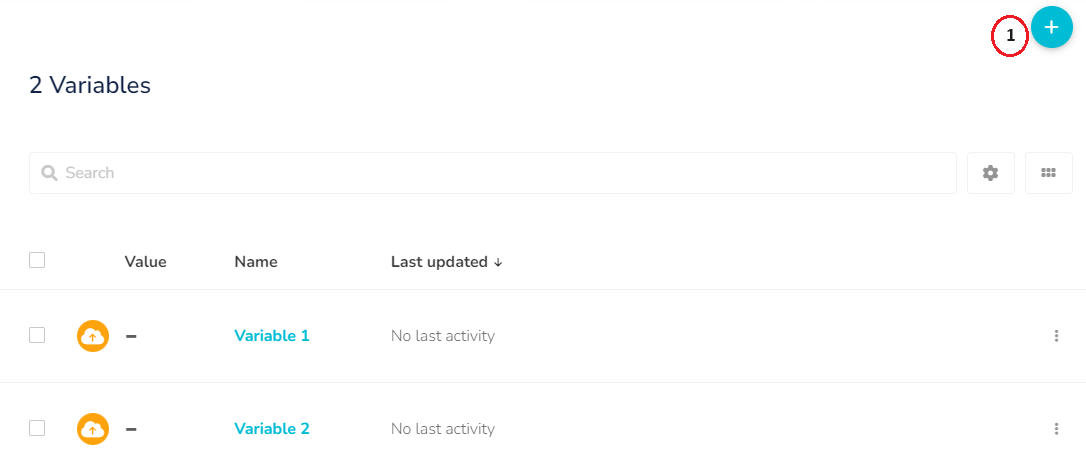
\includegraphics[width=0.7\linewidth]{../images/ubidots_create_variable.png}
		\caption{\label{fig:ubidots_create_variable_1}Creating a variable on Ubidots.}
	\end{figure}
	\item Obtain the API token.
		\begin{figure}[H]
			\centering
			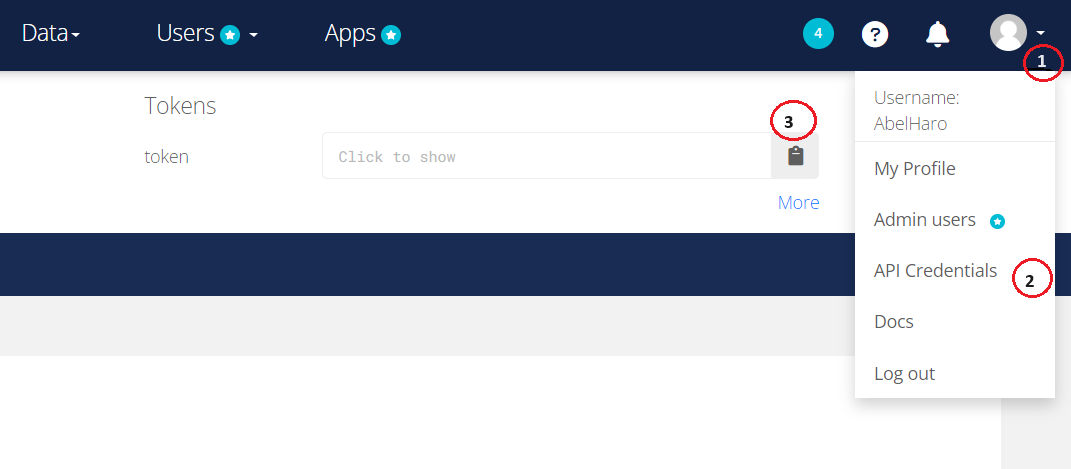
\includegraphics[width=0.7\linewidth]{../images/ubidots_obtener_token.png}
			\caption{\label{fig:ubidots_obtener_token}Obtaining the API token on Ubidots.}
		\end{figure}
	\item Copy the API token to the \texttt{``TOKEN\_UBIDOTS''} variable inside the \texttt{``api/ubidots\_conf.py''} file.
\end{enumerate}

\subsection{Step 2: Circuit Assembly}
For circuit assembly, the following video was used as a reference \href{https://www.youtube.com/watch?v=bvn_o39uXac}{`RFID RC522 with Raspberry Pi Pico and MicroPython Codes for Simple Access Control'} \cite{computadoras2022rfid}.\\
Connect the RFID-RC522 reader to the Raspberry Pi Pico WH following this table:

\begin{center}
	\begin{tabular}{|c|c|}
		\hline
		\textbf{RFID-RC522 Reader} & \textbf{Raspberry Pi Pico WH} \\
		\hline
		VCC & 3.3V \\
		\hline
		RST & GP0 \\
		\hline
		GND & GND \\
		\hline
		IRQ & Not connected \\
		\hline
		MISO & GP4 \\
		\hline
		MOSI & GP3 \\
		\hline
		SCK & GP2 \\
		\hline
		SDA & GP1 \\
		\hline
	\end{tabular}
	\captionof{table}{Connections between the RFID-RC522 reader and the Raspberry Pi Pico WH.}
\end{center}

\vspace{0.3cm}

Connect the KY-016 SP00 tri-color LED to the Raspberry Pi Pico WH following this table:
\begin{center}
	\begin{tabular}{|c|c|}
		\hline
		\textbf{KY-016 SP00} & \textbf{Raspberry Pi Pico WH} \\
		\hline
		R & GP13 \\
		\hline
		G & GP12 \\
		\hline
		B & Not connected \\
		\hline
		- & GND \\
		\hline
	\end{tabular}
	\captionof{table}{Connections between the KY-016 SP00 tri-color LED and the Raspberry Pi Pico WH.}
\end{center}



The circuit assembly should look like the following figure:
\begin{figure}[H]
	\centering
	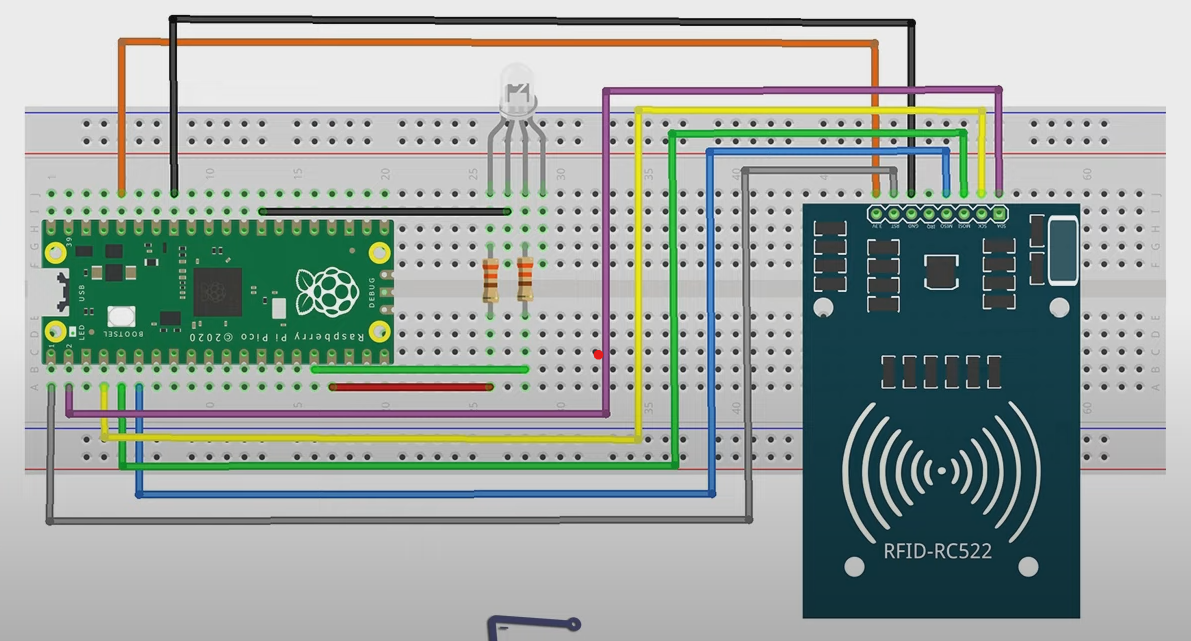
\includegraphics[width=1\linewidth]{../images/esquema_de_conexionado.png}
	\caption{\label{fig:circuito}Project circuit diagram.}
\end{figure}

\subsection{Step 3: Mobile Application Configuration}
To configure the mobile application, follow these steps:
\begin{enumerate}
    \item Install the \href{https://play.google.com/store/apps/details?id=de.kai_morich.serial_usb_terminal&pcampaignid=web_share}{Serial Bluetooth Terminal} app on your mobile device.
    \item Pair the Raspberry Pi Pico WH with the mobile device via Bluetooth.
    \item Open the Serial Bluetooth Terminal app and connect to the Raspberry Pi Pico WH.
    \item Send the message \texttt{``ADD\_USER\_REGISTER''} to the Raspberry Pi Pico WH to change the mode to user registration.
    \item Send the message \texttt{``ADD\_TIME\_REGISTRY''} to the Raspberry Pi Pico WH to change the mode to access registration.
\end{enumerate}
This is how it's shown in the Serial Bluetooth Terminal app:
\begin{figure}[H]
    \centering
    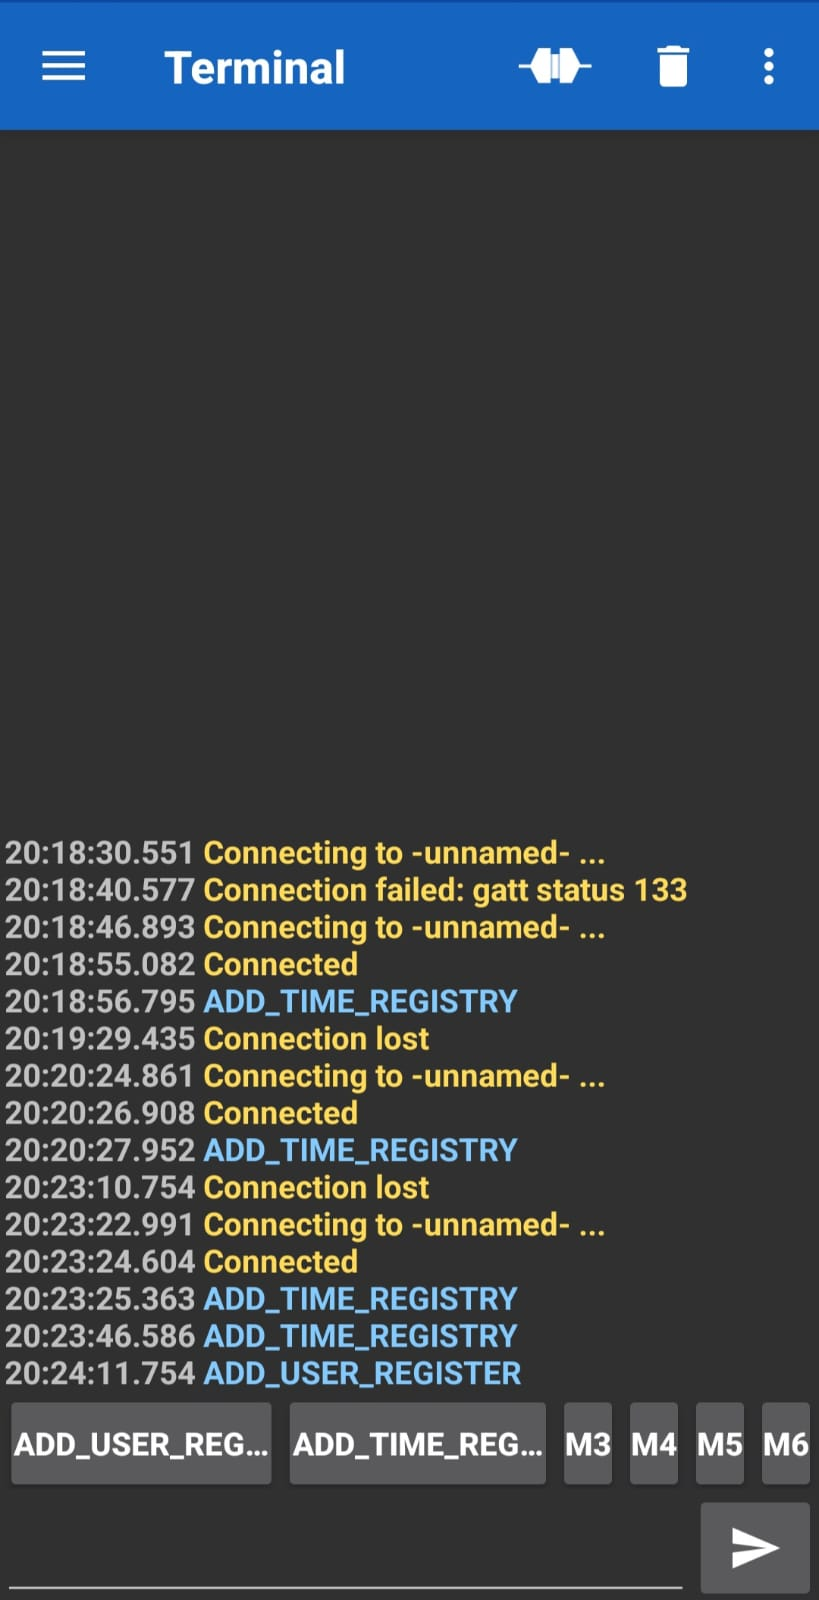
\includegraphics[width=0.5\linewidth]{../images/serial_bluetooth_terminal.jpeg}
    \caption{\label{fig:serial_bluetooth_terminal}Serial Bluetooth Terminal app.}
\end{figure}

\subsection{Step 4: Project Execution}
To execute the project, follow these steps:
\begin{enumerate}
	\item Connect the Raspberry Pi Pico WH to the computer.
	\item Open Thonny and run the \texttt{``microcontroller/main.py''} file on the Raspberry Pi Pico WH.
	\item Start the Docker daemon.
	\item Run the \texttt{``build.bat''} file on the server.
	\item Open Ubidots and visualize the data.
	\item Perform registration and access tests.
\end{enumerate}
This is how it's shown in Ubidots:
\begin{figure}[H]
    \centering
    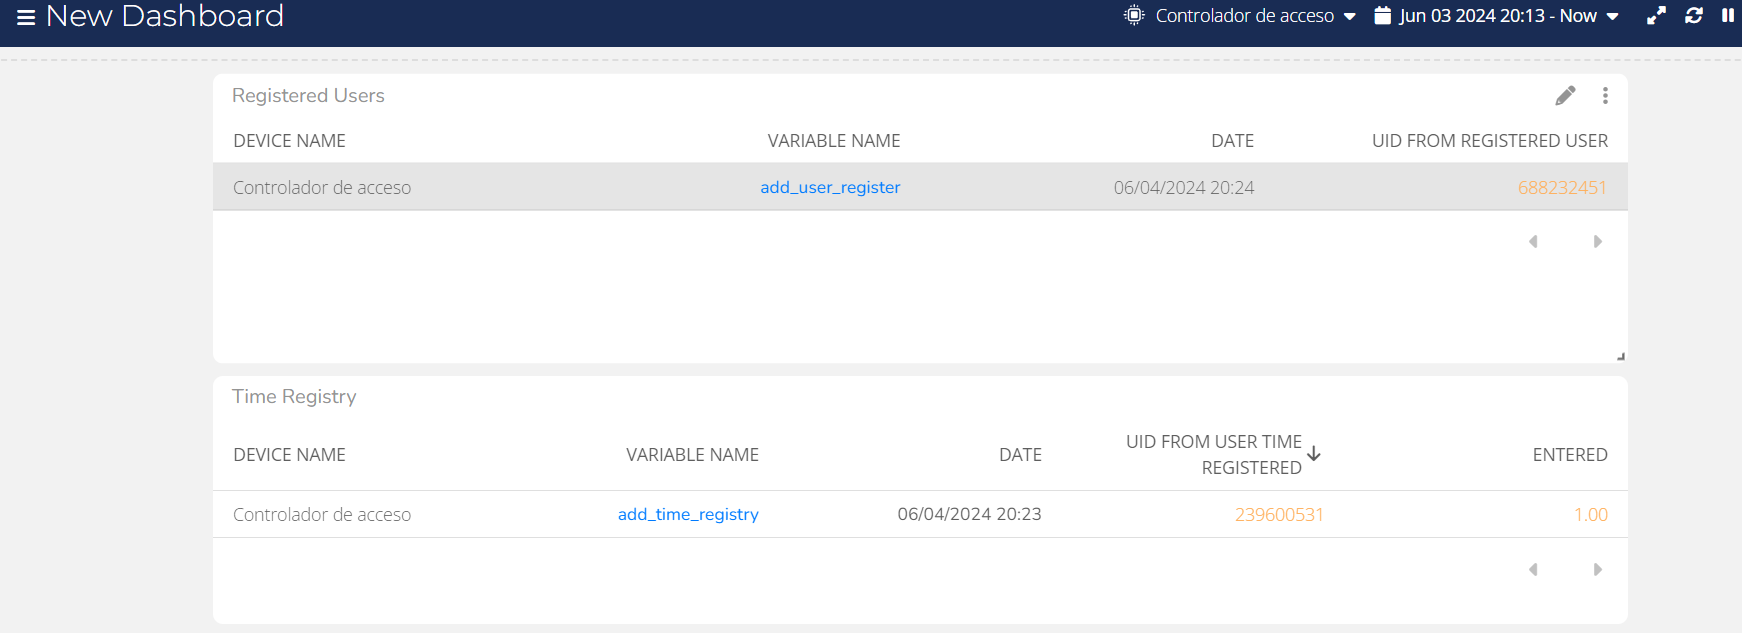
\includegraphics[width=1\linewidth]{../images/ubidots_visualizacion.png}
    \caption{\label{fig:ubidots_visualizacion}Ubidots data visualization.}
\end{figure}

\section{Project Programming}
In this section, the code of the main project files is detailed.

\subsection{Microcontroller}
The microcontroller code is divided into several files:

\subsubsection{main.py}
This file is the main script for the microcontroller. It contains the configuration for Bluetooth communication and the function \texttt{``on\_rx(data)''} where the Bluetooth message is received to change the reading mode.
In the \texttt{``main()''} function, \texttt{``wifi.connect()''} is called to connect to the WiFi network, and the main loop of the program is started.
In the loop, the \texttt{``sensor.read\_sensor()''} function is called to get the UID of the RFID key or card.
If the mode is registration, the \texttt{``sender.add\_user\_register(uid)''} function is called, and if the mode is entry registration, the \texttt{``sender.add\_time\_registry(uid)''} function is called.
Finally, the \texttt{``led.blink\_led(response['api\_status'])''} function is called to turn on the tricolor LED based on the API response.

\begin{lstlisting}
import bluetooth  # Bluetooth module
from ble.ble_simple_peripheral import BLESimplePeripheral  # BLE module
import time
import wifi_connect as wifi
import data_sending_api as sender
import sensor
import led_control as led
import ubidots

# Initialize Bluetooth Low Energy (BLE) interface and Simple Peripheral
ble = bluetooth.BLE()
sp = BLESimplePeripheral(ble, name="Pico WH")

# Default mode for RFID sensor operation
MODE = 'ADD_USER_REGISTER'  # Default mode is to add user registration

def on_rx(data):
    """
    Callback function for receiving data from BLE.

    Parameters:
        data (bytes): Received data as bytes.

    Global Variables Modified:
        MODE (str): Updated mode based on received data.
    """
    global MODE  # Access global variable MODE within the function
    print("Data received:", data)

    # Update mode based on received data
    if data == b'ADD_USER_REGISTER\r\n':
        MODE = 'ADD_USER_REGISTER'
    elif data == b'ADD_TIME_REGISTRY\r\n':
        MODE = 'ADD_TIME_REGISTRY'


if __name__ == '__main__':
    # Connect to WiFi
    wifi.connect()

    try:    
        while True:
            if sp.is_connected():
                sp.on_write(on_rx)  # Register callback for BLE data reception
            # Read UID from sensor
            uid = sensor.read_sensor()
            
            # Determine mode and call appropriate API
            if MODE == 'ADD_USER_REGISTER':
                response = sender.add_user_register(uid)  # Call API to add user registration
            elif MODE == 'ADD_TIME_REGISTRY':
                response = sender.add_time_registry(uid)  # Call API to add time registry
            else:
                print('Error: Invalid mode')
                raise Exception('Invalid mode detected')  # Raise an exception for invalid mode
            
            # Blink LED based on API response status
            led.blink_led(response['api_status'])
            time.sleep(1)
    except KeyboardInterrupt:
        print('Programa abortado con CTRL+C desde main.py')  # Handle keyboard interrupt
\end{lstlisting}
\captionof{figure}{Code for the \texttt{``microcontroller/main.py''} file of the microcontroller.}

\subsubsection{sensor.py}
This file contains the \texttt{``read\_sensor()''} function which reads the RFID sensor and returns the UID of the read RFID key or card.
\begin{lstlisting}
from lib.mfrc522.mfrc522 import MFRC522  # RFID reader module
import time  # Time-related functions
import data_sending_api as sender  # Custom API module for data sending

def read_sensor() -> str:
    """
    Function to read RFID sensor and perform actions based on the received data.

    Returns:
        str: UID from card or key readed.
    """
    # Initialize the MFRC522 RFID reader
    reader = MFRC522(spi_id=0, sck=2, miso=4, mosi=3, cs=1, rst=0)

    print("RFID sensor active...\n")

    try:
        while True:
            reader.init()  # Initialize the RFID reader
            (stat, tag_type) = reader.request(reader.REQIDL)  # Request tag detection

            if stat == reader.OK:
                (stat, uid) = reader.SelectTagSN()  # Select detected tag
                if stat == reader.OK:
                    # Convert UID bytes to integer for identification
                    identifier = int.from_bytes(bytes(uid), "little", False)
                    print("UID: " + str(identifier))  # Print detected UID

                    return str(identifier)  # Convert UID to string
                
            time.sleep(1)  # Sleep for 1 second between iterations

    except KeyboardInterrupt:
        print("Program terminated with CTRL+C from sensor.py")  # Handle keyboard interrupt
\end{lstlisting}
\captionof{figure}{Code of the file \texttt{``microcontroller/sensor.py''} of the microcontroller.}

\subsubsection{data\_sending\_api.py}
This file contains the functions to send data using the server's REST API.
It includes the functions \texttt{``add\_user\_register(uid)''} and \texttt{``add\_time\_registry(uid)''} to send user registration and access data respectively.

\begin{lstlisting}
    import time  # Standard Python time module
    import ujson  # Module for handling JSON data
    import urequests as requests  # Module for making HTTP requests (alias for urequests)
    
    URL = 'http://192.168.1.2:8888/api/'
    URL_add_user_register = URL + 'user_register/add'
    URL_add_time_registry = URL + 'time_registry/add'
    URL_get_user_registered_by_uid = URL + 'user_register'
    
    def get_local_time() -> str:
        """
        Returns the timestamp formatted.
        """
        local_time = time.localtime()
        formatted_time = "{:04d}-{:02d}-{:02d} {:02d}:{:02d}:{:02d}".format(
        local_time[0],  # year
        local_time[1],  # month
        local_time[2],  # day
        local_time[3],  # hour
        local_time[4],  # minute
        local_time[5]   # second
        )
        return str(formatted_time)
    
    def add_user_register(uid):
        """
        Adds the user to the database using a POST request.
        
        Parameters:
            uid (str): The UID (Unique ID) of the user to be registered.
        
        Returns:
            dict: A dictionary containing the response message from the server.
        """
         
        data_sending = {
            "UID": uid,
            "user_creation_tstamp": get_local_time()
        }
        
        response = requests.post(URL_add_user_register, headers={'Content-Type': 'application/json'}, data=ujson.dumps(data_sending))
        return ujson.loads(response.content)
        
    def add_time_registry(uid):
        """
        Adds the time registry to the database using a POST request.
        
        Parameters:
            uid (str): The UID (Unique ID) of the user to be registered.
        
        Returns:
            dict: A dictionary containing the response message from the server.
        """
        data_sending = {
            "UID": uid,
            "user_registry_tstamp": get_local_time()
        }
        
        response = requests.post(URL_add_time_registry, headers={'Content-Type': 'application/json'}, data=ujson.dumps(data_sending))
        return ujson.loads(response.content)
    
    def get_user_registered_by_uid(uid):
        """
        Retrieves user registration details from the server based on UID using a GET request.
        
        Parameters:
            uid (str): The UID (Unique ID) of the user to be registered.
        
        Returns:
            dict: A dictionary containing the response message from the server.
        """
        response = requests.get(URL_get_user_registered_by_uid + '/%s'.format(uid))
        return ujson.loads(response.content)
\end{lstlisting}
\captionof{figure}{Code of the file \texttt{``microcontroller/data\_sending\_api.py''} of the microcontroller.}

\subsection{Server}
\subsubsection{api.py}
This file contains the REST API of the server.
It includes functions to connect to the database, add users and access records, retrieve users and access records based on UID, and send user and access records to Ubidots.
Only the functions for user registration \texttt{``insert\_user\_register()''}, \texttt{``get\_user\_register\_by\_uid(uid)''}, and \texttt{``add\_user\_ubidots(uid)''} are shown in the following figure.

\begin{lstlisting}
    import sqlite3
    from flask import Flask, request, jsonify
    import requests
    from api.ubidots_conf import URL_UBIDOTS, TOKEN_UBIDOTS
    
    ...
    
    def insert_user_register(user):
        """
        Inserts a new user registration record into the 'user_register' table and send it to Ubidots.
    
        Parameters:
            user (dict): Dictionary containing user information with keys:
                         - 'UID': Unique ID of the user.
                         - 'user_creation_tstamp': Timestamp of user creation.
    
        Returns:
            dict: Dictionary containing the status of the operation and error message (if any).
                  Keys:
                  - 'api_status': Boolean indicating the success of the operation.
                  - 'error': Error message if an error occurred during the operation.
                  - 'ubidots_status': HTTP status code of the request to Ubidots.
                  - 'UID': Unique ID of the user.
                  - 'user_creation_tstamp': Timestamp of user creation.
        """
        inserted_user = {'api_status': False, 'error': None, 'ubidots_status': False, 'UID': None, 'user_creation_tstamp': None}
        try:
            conn = connect_to_db()
            conn.row_factory = sqlite3.Row
            cur = conn.cursor()
            cur.execute("SELECT * FROM user_register WHERE UID = ?", (user['UID'],))
            rows = cur.fetchall()
            if len(rows) > 0:
                inserted_user['error'] = "User already exists"
                return inserted_user
            
            cur.execute("INSERT INTO user_register (UID, user_creation_tstamp) VALUES (?, ?)",
                        (user['UID'], user['user_creation_tstamp']) )
            conn.commit()
            inserted_user.update(get_user_register_by_uid(user['UID']))
            ubidots_status = add_user_ubidots(user['UID'])
            if ubidots_status == 200:
                inserted_user['api_status'] = True
            else :
                inserted_user['error'] = "Error adding user to Ubidots"
                
            inserted_user['ubidots_status'] = ubidots_status
        except:
            conn.rollback()
        finally:
            conn.close()
        return inserted_user
    
        def get_user_register_by_uid(uid):
        """
        Retrieves a user record from the 'user_register' table based on the provided UID.
    
        Parameters:
            uid (str): The UID (Unique ID) of the user to retrieve.
    
        Returns:
            dict: A dictionary representing the user record if found, otherwise an empty dictionary.
                  The dictionary contains keys 'UID' and 'user_creation_tstamp' with corresponding values.
        """
        user = {}
        try:
            conn = connect_to_db()
            conn.row_factory = sqlite3.Row
            cur = conn.cursor()
            cur.execute("SELECT * FROM user_register WHERE UID = ?", (uid,))
            rows = cur.fetchall()
    
            # convert row objects to dictionary
            for i in rows:
                user["UID"]  = i["UID"]
                user["user_creation_tstamp"]  = i["user_creation_tstamp"]
                
        except:
            user = {}
        return user
    
        def add_user_ubidots(uid):
        """
        Sends an HTTP POST request to Ubidots API to add a user registration.
    
        Parameters:
            uid (str): The UID (User ID) of the user to register.
    
        Returns:
            int: HTTP status code of the request.
        """
        data = {
            'add_user_register': {
                'value': 1,
                'context': {
                    'UID': uid
                }
            }
        }
        request = requests.post(
            URL_UBIDOTS,
            headers={'X-Auth-Token': TOKEN_UBIDOTS, 'Content-Type': 'application/json'},
            json=data
        )
        return request.status_code
        
        @app.route('/api/user_register/<uid>', methods=['GET'])
        def api_get_user_register_by_id(uid):
            return jsonify(get_user_register_by_uid(uid))
        
        @app.route('/api/user_register/add', methods=['POST'])
        def api_add_user_register():
            user = request.get_json()
            return jsonify(insert_user_register(user))
    
        app.run(host="0.0.0.0")
\end{lstlisting}
\captionof{figure}{Code of the file \texttt{``api/api.py''} of the server.}

\subsubsection{initdb.py}
This file contains the initialization of the database.
It creates the \texttt{``database''} directory if it does not exist and the \texttt{``database.db''} file if it does not exist.
It creates the \texttt{``user\_register''} and \texttt{``time\_registry''} tables if they do not exist.

\begin{table}[H]
	\centering
	\begin{tabular}{|l|l|l|}
	\hline
	\textbf{Column Name} & \textbf{Data Type} & \textbf{Constraints} \\ \hline
	\texttt{UID} & \texttt{TEXT} & \texttt{PRIMARY KEY, NOT NULL} \\ \hline
	\texttt{user\_creation\_tstamp} & \texttt{TEXT} & \texttt{NOT NULL} \\ \hline
	\end{tabular}
	\caption{Table \texttt{user\_register} schema.}
	\end{table}

\begin{table}[H]
	\centering
	\begin{tabular}{|l|l|p{8cm}|}
	\hline
	\textbf{Column Name} & \textbf{Data Type} & \textbf{Constraints} \\ \hline
	\texttt{id} & \texttt{INTEGER} & \texttt{PRIMARY KEY AUTOINCREMENT} \\ \hline
	\texttt{user\_registry\_tstamp} & \texttt{TEXT} & \texttt{NOT NULL} \\ \hline
	\texttt{UID} & \texttt{TEXT} & \texttt{NOT NULL, REFERENCES user\_register(UID)} \\ \hline
	\end{tabular}
	\caption{Table \texttt{time\_registry} schema.}
	\end{table}
```
\begin{lstlisting}
import sqlite3
import os

if __name__ == '__main__':
    try:
        # Create the directory if it doesn't exist
        os.makedirs('database', exist_ok=True)
        print("Database directory created successfully.")

        # Create the database file if it doesn't exist
        open('database/database.db', 'a').close()
        print("Database file created successfully.")

        # Establish connection to the database
        conn = sqlite3.connect('database/database.db')
        print("Connection to the database established successfully.")

        # Create user_register table
        conn.execute('''
                    CREATE TABLE IF NOT EXISTS user_register (
                        UID    TEXT PRIMARY KEY NOT NULL,
                        user_creation_tstamp TEXT NOT NULL
                    )
        ''')
        print("Table 'user_register' created successfully.")

        # Create time_registry table
        conn.execute('''
                    CREATE TABLE IF NOT EXISTS time_registry (
                        id INTEGER PRIMARY KEY AUTOINCREMENT,
                        user_registry_tstamp TEXT NOT NULL,
                        UID TEXT NOT NULL REFERENCES user_register(UID)
                    )
         ''')

        print("Table 'time_registry' created successfully.")

        # Commit changes
        conn.commit()
        print("Changes committed successfully.")
    except Exception as e:
        print(e)
        print("Table creation failed")
    finally:
        conn.close()

\end{lstlisting}
\captionof{figure}{Code of the file \texttt{``api/initdb.py''} of the server.}

\subsubsection{build.bat, Dockerfile, and start.sh}
These files are necessary for creating the Docker container for the server.
The file \texttt{``build.bat''} contains the commands for building the image and starting the container.
The file \texttt{``api/Dockerfile''} contains the instructions for building the container image.
The file \texttt{``api/start.sh''} contains the instructions for initializing the database and running the API.


\begin{lstlisting}
	REM Change directory to the location of the Dockerfile
	cd ./api
	
	REM Build Docker image
	docker build -t server_rfid .
	
	REM Run Docker container
	docker run --rm -it -v database:/home/database -p 8888:5000 --name server_rfid server_rfid	
\end{lstlisting}
\captionof{figure}{Code of the file \texttt{``build.bat''} of the server.}

\begin{lstlisting}
FROM ubuntu

# Instalar Python 3 y Flask
RUN apt update
RUN apt install python3 python3-pip -y
RUN apt install python3-flask -y
RUN apt install python3-requests -y

# Establecer el directorio de trabajo y copiar los archivos
WORKDIR /home/
COPY initdb.py .
COPY api.py .
COPY start.sh .
COPY ubidots.py .

# Dar permisos para ejecutar el script
RUN chmod +x start.sh

# Exponer el puerto
EXPOSE 5000

# Ejecutar los scripts
CMD ["./start.sh"]

\end{lstlisting}
\captionof{figure}{Code of the file \texttt{``api/Dockerfile''} of the server.}

\begin{lstlisting}
	#!/bin/sh

# Check if the database directory exists, if not, create it (Only for the first run)
if [ ! -d "database" ]; then
    mkdir database
fi

# Initialize the database
python3 initdb.py

# Start the API
python3 api.py
\end{lstlisting}
\captionof{figure}{Code of the file \texttt{``api/start.sh''} of the server.}

\subsubsection{ubidots\_conf.py}
This file contains the configuration of Ubidots.
It includes the Ubidots URL, device, and API token.
\begin{lstlisting}
DISPOSITIVE_NAME = '' # Device name in Ubidots
URL_UBIDOTS = f'http://industrial.api.ubidots.com/api/v1.6/devices/{DISPOSITIVE_NAME}/'
TOKEN_UBIDOTS = '' # Token of the API
\end{lstlisting}
\captionof{figure}{Code from the file \texttt{``api/ubidots\_conf.py''} on the server.}

\section{Issues Encountered}

The following sections describe the issues encountered during the project and the proposed solutions:

\subsection{Problem 1: Static Server Address}

In order to access the server from the Raspberry Pi Pico WH consistently without having to modify the code, a static IP address must be set for the server. 
This can be achieved by configuring the router's DHCP settings.

Access the router's configuration page using a web browser. 
Typically, this can be done by entering the router's IP address, in my case 192.168.1.1, in the address bar and logging in with the username \texttt{``admin''} and the password. 
Once logged in, navigate to the advanced configuration or DHCP settings section to assign a static IP address to the server. 
In my case, as shown in Figure \ref{fig:configuracion router}, the router dynamically assigns IP addresses to devices connected in the range of 192.168.1.10 - 192.168.1.150. 
Therefore, the IP address 192.168.1.2 was assigned to the server to ensure it always has the same IP address and does not collide with other devices.

\begin{figure}[H]
    \raggedright
    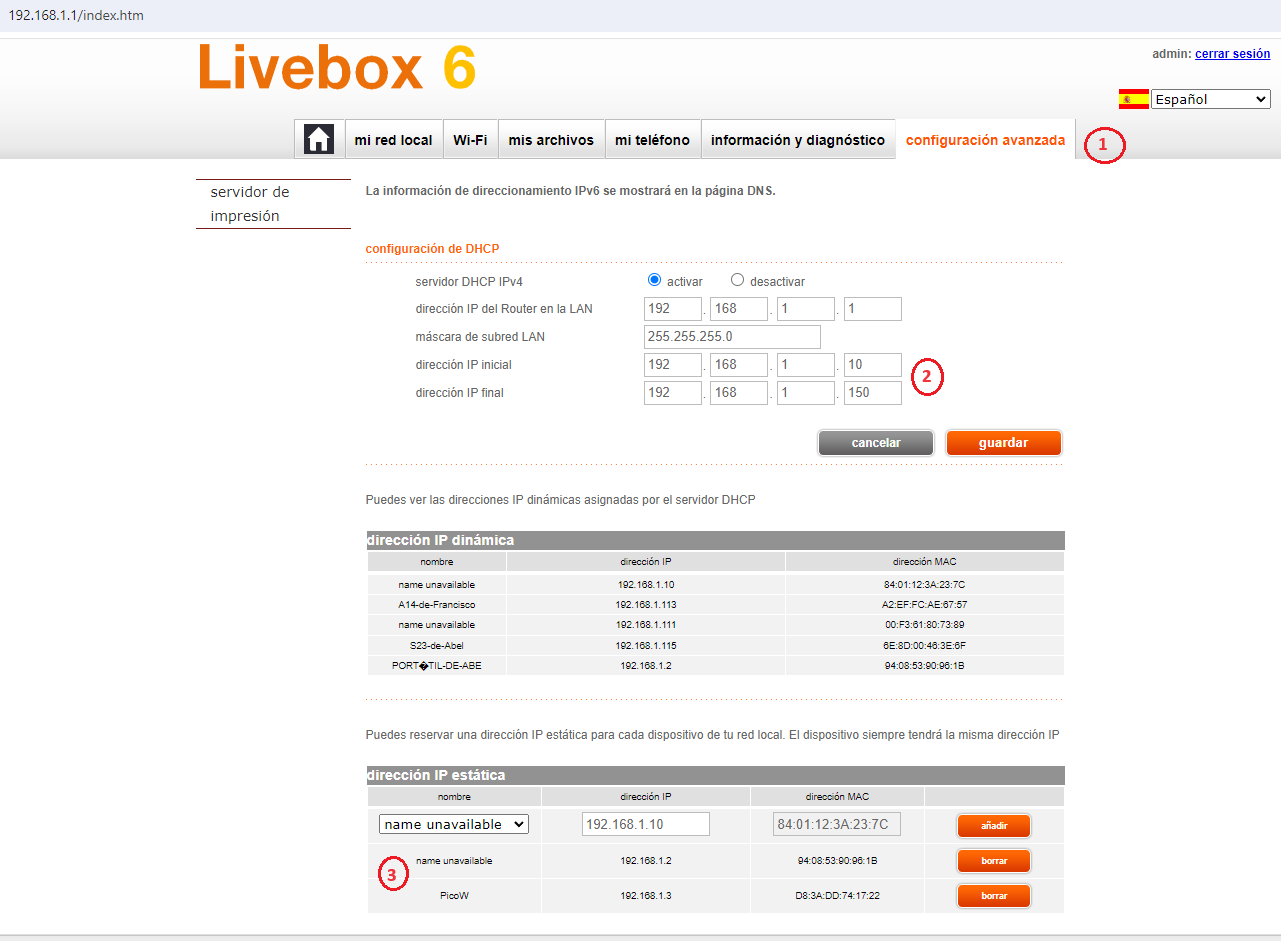
\includegraphics[width=1\linewidth]{../images/router_config.png}
    \caption{\label{fig:configuracion router}Router network configuration.}
\end{figure}

\subsection{Problem 2: Docker Volume}

To maintain database data persistently, a Docker volume must be created. In the Docker Desktop application, navigate to the \texttt{``Volumes''} option and create a volume named \texttt{``database''} as shown in Figure \ref{fig:volumen docker}.

\begin{figure}[H]
    \raggedright
    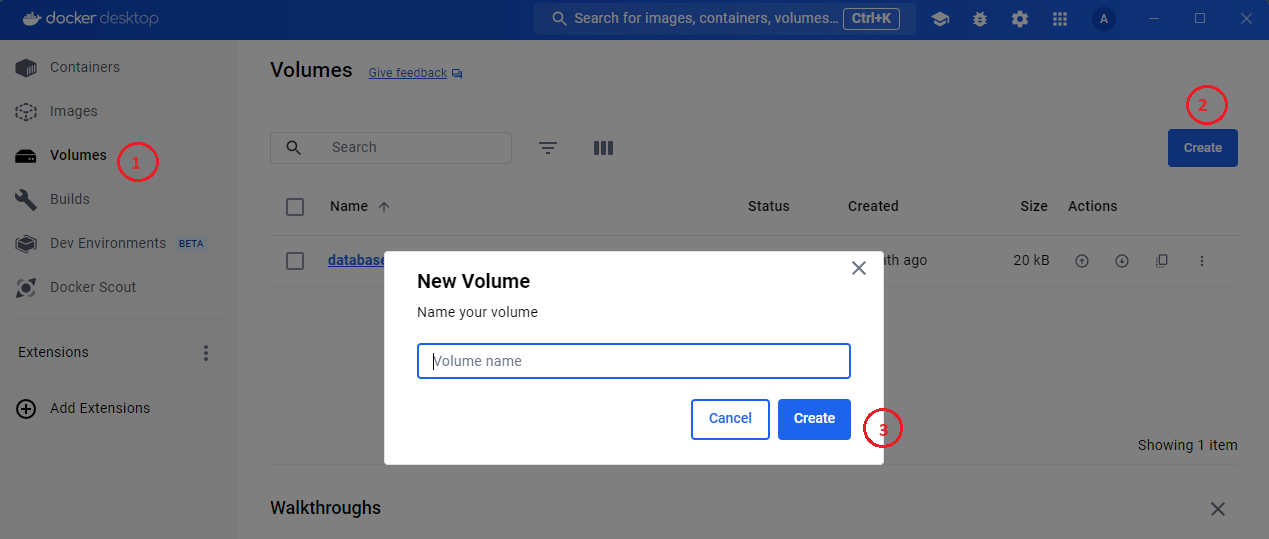
\includegraphics[width=1\linewidth]{../images/volumen_docker.png}
    \caption{\label{fig:volumen docker}Creating a Docker volume.}
\end{figure}

In the \texttt{``build.bat''} file, the volume is linked to the container using the command \texttt{``-v database:/home/database''}.

\subsection{Problem 3: Sending Data to Ubidots}

To send data to Ubidots, the device must be configured in Ubidots and the API token must be obtained. The API token must be sent in the HTTP request header. To do this, refer to the Ubidots documentation to find the request format and send the data in the correct format with the \texttt{``X-Auth-Token''} header.

\begin{lstlisting}
def add_user_ubidots(uid):
    ...
    request = requests.post(
        URL_UBIDOTS,
        headers={'X-Auth-Token': TOKEN_UBIDOTS, 'Content-Type': 'application/json'},
        json=data
    )
    ...
\end{lstlisting}
\captionof{figure}{Code for sending data to Ubidots from the file \texttt{``api/api.py''}.}


\section{Results Obtained}

A access control system using RFID keys and cards has been successfully implemented with a Raspberry Pi Pico WH microcontroller and a server with a SQLite database and a REST API. 

User registration and access data has been successfully sent to Ubidots for real-time visualization. The reading mode of the RFID key or card has been successfully changed using Bluetooth Low Energy. A tricolor LED has been successfully turned on based on the API response. 

The application has been successfully tested and user registration and access have been correctly recorded. 

Future work includes improving the system's security by encrypting data and scalability of the system with multiple Raspberry Pi Pico WHs and RFID readers communicating with the server. The technology for reading RFID keys and cards could also be changed to NFC, a facial recognition system, or fingerprint recognition to enhance the system's security.

\addcontentsline{toc}{section}{References} % Add the References section to the table of contents
\bibliographystyle{plain}
\bibliography{refs}



\end{document}
